\clearpage
\newpage
\subsubsection{Estensione C: Errore Durante la Pubblicazione dell'Annuncio}

Nel caso in cui si verifichi un errore durante la pubblicazione dell'annuncio immobiliare, viene mostrato un popup informativo che comunica all'utente il problema riscontrato. Questo popup ha il compito di rassicurare l'utente che i dati inseriti non andranno persi, in quanto vengono salvati localmente, e invita a riprovare più tardi.

\subsubsection{Gestione dell'Errore e Feedback Utente}
Il popup presenta i seguenti elementi chiave:
\begin{itemize}
    \item \textbf{Messaggio chiaro e rassicurante}: informa l'utente dell'errore senza tecnicismi, riducendo il senso di frustrazione.
    \item \textbf{Pulsante “Riprova”}: consente di tentare nuovamente la pubblicazione con un'animazione di caricamento, per segnalare che l'azione è in corso e mantenere un senso di controllo e progressione.
    \item \textbf{Pulsante “Monstra i Dettagli”}: offre la possibilità di visualizzare l'errore tecnico riscontrato. Questa funzione segue i principi di trasparenza e controllo dell'utente, utili sia per utenti avanzati che per eventuali tecnici di supporto che potrebbero risolvere il problema più rapidamente.
\end{itemize}

\subsubsection{Principi di Design Applicati}
L'implementazione di questa gestione degli errori si basa su diversi principi della UX e dell'usabilità:
\begin{itemize}
    \item \textbf{Visibilità dello stato del sistema} \cite{nielsen1995}: l'animazione di caricamento fornisce un'indicazione chiara che il sistema sta lavorando sulla richiesta dell'utente.
    \item \textbf{Prevenzione degli errori} \cite{nielsen1995}: il salvataggio locale dei dati riduce la possibilità di perdere informazioni a causa di un problema temporaneo.
    \item \textbf{Fornire informazioni utili per il recupero dall'errore} \cite{nielsen1995}: il messaggio di errore è accompagnato da suggerimenti su come procedere e un'opzione per visualizzare i dettagli tecnici, utile per il supporto tecnico.
\end{itemize}

Queste soluzioni mirano a mantenere un'esperienza utente fluida e priva di frustrazione, minimizzando il disagio derivante da problemi tecnici imprevisti.


\begin{figure}[ht]
    \centering
    \begin{tikzpicture}[node distance=1.5cm and 1cm, auto]
        % Nodo per immagine 1 con didascalia sotto
        \node (img1) {
            \begin{tabular}{c}
                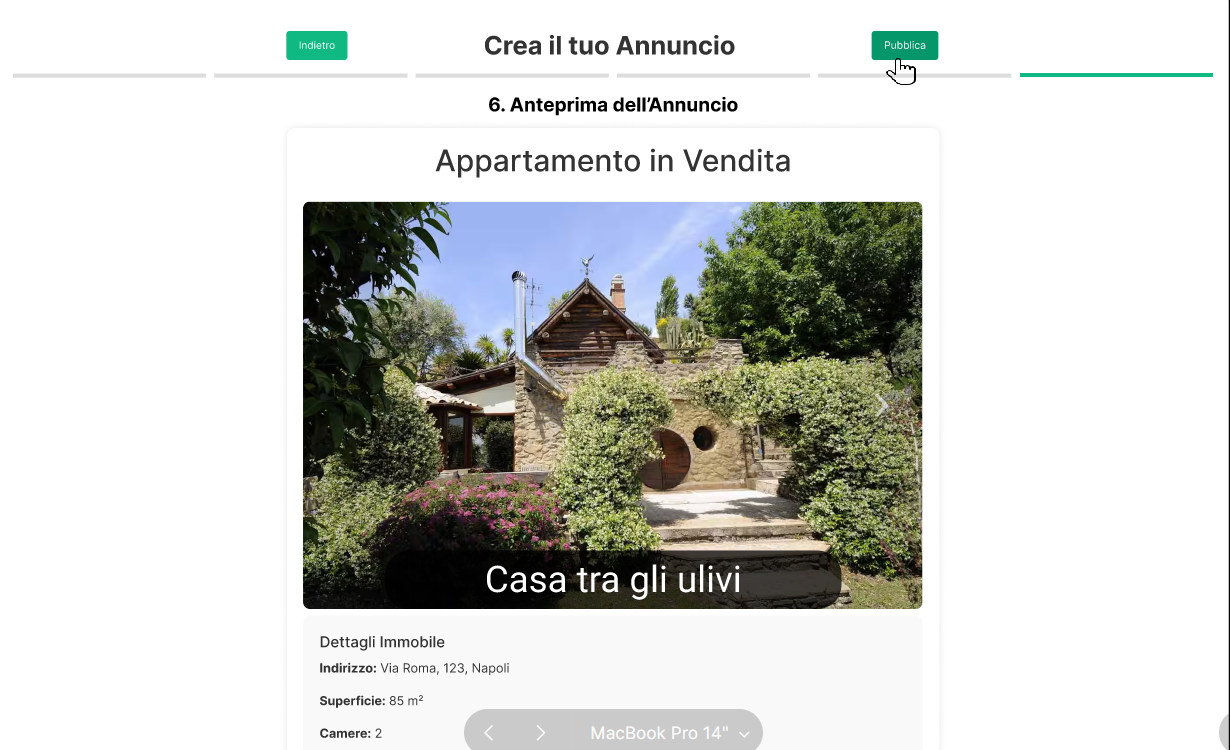
\includegraphics[width=0.7\textwidth]{Immagini/Mockup/aggiungi annuncio/estensione C/step1.png} \\
                click pubblica nuovo annuncio
            \end{tabular}
        };
        
        % Nodo per immagine 2 con didascalia sotto, posizionato a destra di img1
        \node (img2) [below=of img1] {
            \begin{tabular}{c}
                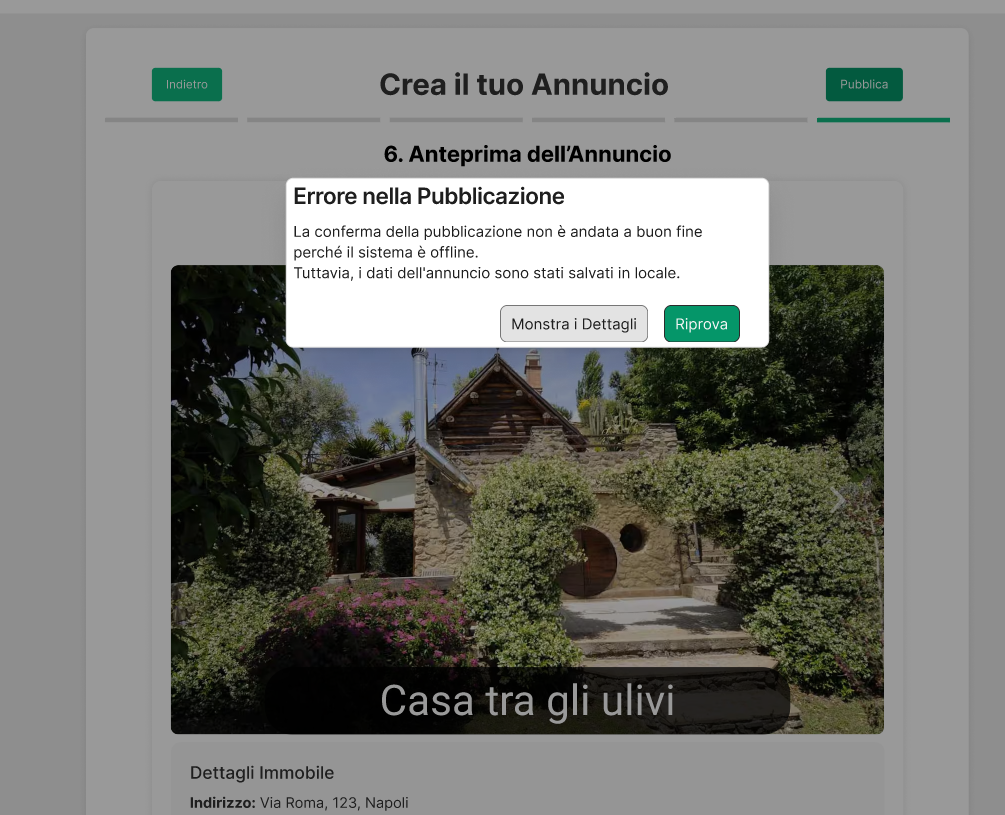
\includegraphics[width=\textwidth]{Immagini/Mockup/aggiungi annuncio/estensione C/step2.png} \\
                Cockburn: extension C.9/C.10
            \end{tabular}
        };
        
        
        % Disegna le frecce
        \draw[->, thick] (img1) -- (img2);
      
    \end{tikzpicture}
    \caption{Mockup: estensione C della tabella di Cockburn del caso d'uso nuovo annuncio}
    \label{fig:tikz_flow}
\end{figure}

\newpage

